\documentclass[11pt,letterpaper]{article}
\usepackage[top=1in,bottom=1in,left=1in,right=1in]{geometry}
\usepackage[numbers]{natbib}      % http://merkel.zoneo.net/Latex/natbib.php
\usepackage{lmodern}
\renewcommand\familydefault{\sfdefault} 
\usepackage[T1]{fontenc}

%\bibpunct{(}{)}{;}{a}{,}{,}
\usepackage{chngpage}
\usepackage{stmaryrd}
\usepackage{amssymb}
\usepackage{amsmath}
\usepackage{amsthm}
\usepackage{graphicx}
\usepackage{lscape}
\usepackage{subfigure}
\usepackage{parskip}
\usepackage{algpseudocode}
\usepackage{algorithm}
\usepackage[usenames,dvipsnames]{color}
\usepackage{indentfirst}
\definecolor{myblue}{rgb}{0,0.1,0.6}
\definecolor{mygreen}{rgb}{0,0.3,0.1}
\usepackage[colorlinks=true,linkcolor=black,citecolor=mygreen,urlcolor=myblue]{hyperref}
\newcommand{\bocomment}[1]{\textcolor{Bittersweet}{[#1 -BTO]}}
\newenvironment{itemizesquish}{\begin{list}{\labelitemi}{\setlength{\parskip}{0.6cm}\setlength{\itemsep}{0em}\setlength{\labelwidth}{2em}\setlength{\leftmargin}{\labelwidth}\addtolength{\leftmargin}{\labelsep}}}{\end{list}}
\newcommand{\norm}[1]{\left\lVert#1\right\rVert}
\newcommand{\ignore}[1]{}
\let\oldReturn\Return
\renewcommand{\Return}{\State\oldReturn}

\theoremstyle{definition}
\newtheorem{question}{Question}[section]

\setlength{\parindent}{30pt}
\linespread{1}

\title{
Protein sequence classification using neighbor-joining\\
   CMSC 701 Final report
}

\author{
	Khanh Nguyen and Ugur Koc
}

\begin{document}
\maketitle

\section{Introduction}

Neighbor-joining algorithm (NJ) is a widely used algorithm for reconstructing phylogenetic trees from evolutionary distance data. The method takes a greedy bottom-up approach, iteratively joining pairs of taxonomic units that minimizes pre-computed distances. In this work, we present our C++ implementation of the algorithm. We compare the running time of the implementation with other popular packages. In addition, we also provide a benchmark on our implementation for computing the distance matrix between sequences. We found our implementation is able to produce phylogenetic trees with high accuracy, and it does so faster than some highly-used molecular biology (i.e. phylogenetic) programs. TODO rephrase

\section{Background}

%\subsection{Hierarchical clustering}

\subsection{Phylogenetic trees}

\begin{figure}[h]
  \centering
  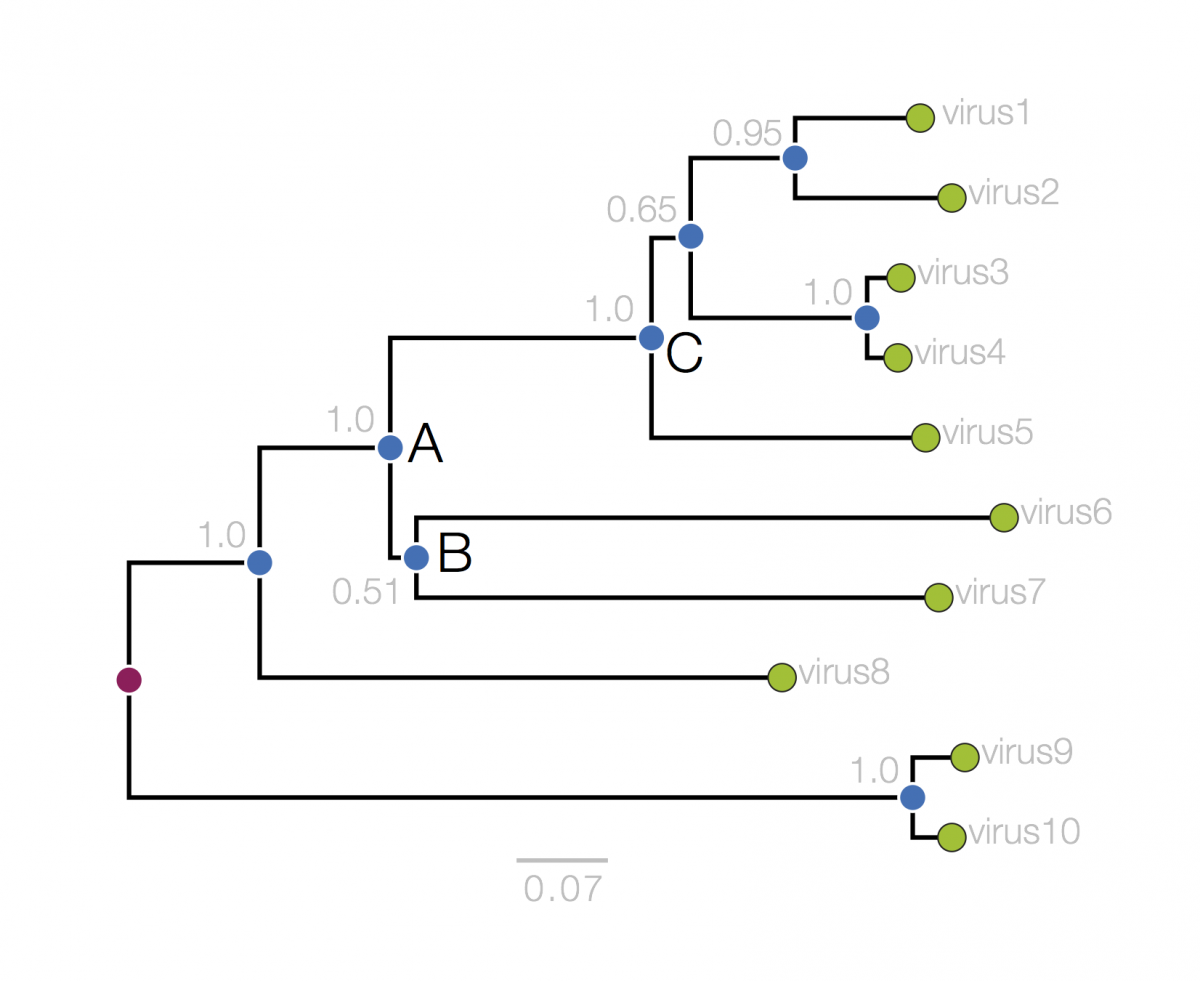
\includegraphics[width=0.6\textwidth]{phylogram_1a.png}
  \caption{An example of phylogenetic tree.}
  \label{fig:phytree}
\end{figure}

Phylogenetic trees are branching diagrams that show the evolutionary relationships between biological species. A weighted phylogenetic tree, with weights associated with its edges, captures the notion of genetic distances between species. By analyzing a weighted phygenetic tree, we understand not only \textit{how} but also \textit{how much} species are related to or different from one another. Figure \ref{fig:phytree} \footnote{Image taken from \url{http://epidemic.bio.ed.ac.uk/how_to_read_a_phylogeny}} features an artificial phylogentic tree of 10 viruses. Each virus is represented by a leave in the tree. Each internal node marks a milestone when a genetic divergence occurs. The lengths of the horizontal lines represent time periods. For instance, we can see that the divergence between virus 1 and virus 2 occurs before the divergence between virus 3 and virus 4. Phylogentic trees can be constructed from various distance metrics. In this example, the metric assigned to the edges is the proportion of substitutions occuring on a sequence (the number of substituions divided by the length of the sequence). 

\subsection{Neighbor-joining algorithm}

We consider the problem of constructing a phylogentic tree from a set of protein sequences given their distance data. There are many approaches to tackle this problem. One approach frames the problem as as a hierarchical clustering problem, which has been extensively studied in the fields of data mining or machine learning and has efficient solutions using statistical models. Although statistical approaches methods have been employed to build these complex evolution trees, classical approaches such as the NJ algorithm has the advantage of being easy to implement and scalable to large datasets. 

Figure \ref{alg:nj} summarizes the NJ algorithm. The input for the NJ algorithm are a set $P$ of sequences (usually DNA or protein sequences) and a distance matrix $D$ where each entry is the distance between a pair of sequences. The NJ algorithm constructs the phylogentic tree from bottom up, going from leaves to root. It starts with a forest of $N$ single-node trees, each of which represents a sequence. In each later step, the algorithm selects two trees in the forest, joins them into a single tree by connecting their roots to a newly formed root. This process repeats until there is only tree left in the forest.

In an intermediate step, the algorithm decides which two trees to join by computing a \textit{branch length} matrix $L$ based on the distance matrix $D$. The branch length matrix contains $T \times T$ entries, where $T$ is the number of trees in the forest at the current step. Each entry of the matrix is computed as follows:  
\begin{equation}
  L_{i, j} = (T - 2) D_{i, j} - \sum_{k \in R}^n (D_{i, k} + D_{j, k})
  \label{eqn:branch}
\end{equation} where $R$ is the set of tree roots in the current forest.

Next, the algorithm selects the pair ($x$, $y$) with the highest branching length and connects each node to a new root, say $u$. The distances between u and x, y are:  
\begin{equation}
\begin{split}
  & D_{u, x}^{'} = \frac{1}{2} D_{x, y} + \frac{1}{2(T - 2)} \left[ \sum_{k \in R} (D_{x, k} - D_{y, k}) \right] 
\\  
& D_{u, y}^{'} = D_{x, y} - D_{u, x}^{'}
\end{split}
\label{eqn:distance_joined}
\end{equation}

We also update the distances between $u$ and other roots:
\begin{equation}
  D_{u, z}^{'} = \frac{1}{2} \left[ D_{x, z} + D_{y, z} - D_{x, y} \right], \ \ \ \text{for} \ z \neq x, y
\label{eqn:distance_nonjoined}
\end{equation}

\begin{figure}
  \begin{algorithmic}[1]
    \Function{Neighor-joining}{$P$, $D$}
      \State $T \leftarrow \varnothing$ 
      \State $R \leftarrow P$
      \For {$t = 1 \dots |P| - 2$}
        \State $T \leftarrow |R|$
        \For {$(i, j) \in R \times R$}
          \State Compute $L_{i, j}$ using equation \ref{eqn:branch}. 
        \EndFor
        \State $(x, y) \leftarrow \arg \max L$
        \State Create new root $u$.
        \State Compute $D^{'}$ from $u$ to other nodes using equations \ref{eqn:distance_joined} and \ref{eqn:distance_nonjoined}.
        \State $D \leftarrow D^{'}$
        \State $T \leftarrow T \cup \{(u, x, D_{u, x}), (u, y, D_{u, y})\}$
        \State $R \leftarrow R \cup \{u\} \setminus \{x, y\}$
      \EndFor
    \State Let $u, v$ be the only two elements left in $R$.
    \State $T \leftarrow T \cup \{(u, v, D_{u, v})\}$
    \Return $T$
   \EndFunction
  \end{algorithmic}
  \caption{\label{alg:nj}The neighbor-joining algorithm.}
\end{figure}



\subsection{Computing distance matrix}\label{distance}

Neighbor-joining algorithm is deterministic, i,e, given a distance matrix it will always produce the same phylogenetic tree. Therefore, computing accurate phylogenetic trees highly depends on the model of evaluation, i,e, distance matrix.

In this project we tried three different ways to generate the distance matrix.
\begin{itemize}
	\item Using \textit{distmat} program from emboss package\footnote{\url{http://emboss.sourceforge.net/apps/release/6.6/emboss/apps/distmat.html}} which computes distance matrix for already aligned sequences~\cite{rice2000emboss}. We wrote a wrapper script in perl to call this program and then post process it's output in order to put it in the format of input distance matrix of our NJ implementation (see \textit{aligntodist.pl} script in source code).
	\item Using \textit{protdist} program from phylibpackage\footnote{\url{http://evolution.genetics.washington.edu/phylip.html}} which again computes  distance matrix for already aligned sequences~\cite{plotree1989phylip}. We slightly modified the source code in order to have the output in required format and we also removed some unnecessary functionality which does not matter for this project (see \textit{protdist.c} source file for details).
	\item Lastly, computing global alignment scores for each pair of sequences and using geometric inverse of that score as distance. To do this we wrote two scripts; \textit{pairwisealignment.sh} and \textit{aligntodist\_pw.pl}. First script creates the global alignment scores for each pair and the second one computes the distance matrix from them.
\end{itemize}

\section{Experiments}

To evaluate the effectiveness and the efficiency of our implementations, we conducted a set of experiments. 

We first aimed at generating accurate phylogenetic tree trying out different approaches (evaluation models) when generating the distance matrix. We then compared our results with some other popular implementations of neighbor-joining algorithm. 

In these experiments, effectiveness refers to the accuracy of the phylogenetic tree produced at the end, i.e. how close/similar the tree to the ground truth by comparing them using robinson foulds symmetric difference \cite{robinson1981comparison}, and the efficiency refers to 1) the computation time of distance matrix and 2) computation of phylogenetic tree.

\subsection{Data}

In all experiments, we used a dataset which is consist of 85 protein sequences of fully sequenced species representing all major Eukaryotic lineages. We took this dataset and the corresponding phylogenetic tree from\footnote{See Additional File 5 and 6 \url{http://www.biomedcentral.com/1471-2105/15/222}} \cite{khafif2014identification}. The longest sequence in this set has 125 amino acids. The phylogenetic tree has nine major branches which groups families of Eukaryotic lineages together. We considered this tree as the ground truth when comparing different distance matrix generation approaches.

\subsection{Results}

As results of our experiments we produced; 1) global alignment files, 2) distance matrix files, and 3) phylogenetic tree files in \textit{newick} format. These files can be found under data directory. 

\subsubsection{Study 1; Generating accurate phylogenetic tree}

Here, we compare effectiveness and efficiency of three different approaches mentioned in Section~\ref{distance}. Time values in the following tables and measured in seconds and the accuracy is computed as the norm of robinson foulds symmetric difference~\cite{robinson1981comparison}. 

\begin{table}[!h]
\centering
	\begin{tabular}{l|lll|lll|lll}

Gap Score	& \multicolumn{3}{c}{g=1} & \multicolumn{3}{c}{g=25} &  \multicolumn{3}{c}{g = 75} \\
\hline
&	$T_d$	& $T_{NJ}$	& accuracy &	$T_d$	& $T_{NJ}$	& accuracy &	$T_d$	& $T_{NJ}$	& accuracy \\
\hline
Uncorrected		&	0.091	&	0.008	&	0.390	&	0.088	&	0.009	&	0.524	&	0.090	&	0.008	&	0.622	\\
Jukes-Cantor	&	0.089	&	0.008	&	0.463	&	0.089	&	0.010	&	0.549	&	0.090	&	0.009	&	0.829	\\
Kimura Protein	&	-	&	-	&	-	&	-	&	-	&	-	&	0.115	&	0.009	&	0.915	\\
\hline
\end{tabular}
\caption{Performance of evolution models implemented in \textit{distmat}. 
$T_d$; time to compute distance matrix and $T_{NJ}$; time to compute the phylogenetic tree (both are in seconds), and accuracy is computed using robinson foulds symmetric difference \cite{robinson1981comparison} (norm\_rf)}\label{tab:dist1}
\end{table}

\textbf{Performance of \textit{distmat} methods}. \textit{distmat} has tree different multiple substitution correction methods implemented for aligned proteins sequences. They are Uncorrected, Jukes-Cantor~\cite{jukes1969evolution}, and Kimura Protein~\cite{kimura1980simple}. Table~\ref{tab:dist1}  presents computation times and the phylogenetic tree accuracy scores for these methods (Kimura Protein evolution model does not make use a gap score, thus it only has one set of results).

\begin{table}[!h]
\centering
	\begin{tabular}{l|lll}
	\hline
	&	$T_d$	& $T_{NJ}$	& accuracy  \\
	\hline
	Dayhoff PAM	&	3.867	&	0.010	&	0.390	\\
	JTT			&	3.809	&	0.009	&	0.378	\\
	PMB			&	3.934	&	0.012	&	0.341	\\
	Kimura		&	0.013	&	0.012	&	0.963	\\
	\hline
	\end{tabular}
\caption{Performance of evolution models implemented in \textit{protdist}. 
$T_d$; time to compute distance matrix and $T_{NJ}$; time to compute the phylogenetic tree (both are in seconds)}\label{tab:dist2}
\end{table}

\textbf{Performance of \textit{protdist} methods}. \textit{protdist} has five method for amino-acid substitutions, but we have only experimented with four of them. They are namely, Dayhoff PAM matrix~\cite{kosiol2005different}, Jones-Taylor-Thornton model (JTT)~\cite{jones1992rapid}, PMB (Probability Matrix from Blocks) model~\cite{veerassamy2003transition}, and the Kimura's distance~\cite{kimura1983rare}. Table~\ref{tab:dist2} presents computation times and the phylogenetic tree accuracies for these methods.

The dataset we used was already aligned, i.e. multiple sequence alignment. As a last part of this study we revert this alignment to a set of sequences and then compute a global alignment score of each pair of sequences in this set. Our motivation was to see if global alignment scores can be effective in generating a distance matrix. Scoring system we used in global alignment gave higher scores to better alignments (substitution matrix: EBLOSUM62, gap penalty: 10.0, and gap extend penalty: 0.5). We therefore took geometric inverse of of these alignment scores and then multiplied them by 1000. Result is the used as the distance between those sequences.

Computing global alignment was very time consuming (it took 30mins roughly). However, other distance matrix generation approaches took multiple sequence alignments as input. That sequence alignment was done in~\cite{khafif2014identification}, and we don't know how much time it took to compute it. We therefore do not include cost of pairwise global alignment it our evaluation. Given global alignments (scores) computing the distance matrix took 0.221 seconds, our NJ implementation took 0.011 second to generate the phylogenetic tree and the accuracy (robinson foulds metric) of that tree was 0.634.

Based on the results given in Table \ref{tab:dist1}, \ref{tab:dist2}, and previous paragraph, we can say that our NJ implementation is very efficient, i.e. computation of the tree is very fast (for the dataset we worked on) and does not depend on distance matrix generation approach. Effectiveness however depends on the approach and the gap score. We achieved our the best phylogenetic tree with Kimura Protein evolution model. And for Uncorrected and Jukes-Cantor models accuracy of the tree increased as the gap score increased.

\subsubsection{Study 2; Comparing with other neighbor-joining implementations}

\begin{figure}[t]
  \centering
  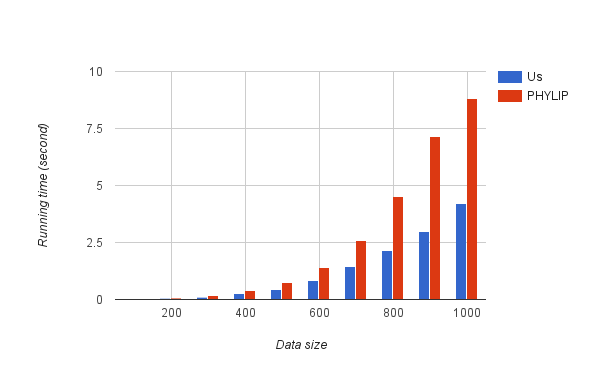
\includegraphics[width=0.9\textwidth]{runningtime.png}
  \caption{Comparison on the running times of our NJ implementation and PHYLIP's.}
  \label{fig:runningtime}
\end{figure}


We present both qualitative and quantitative comparisions between our NJ implementation and that of the PHYLIP package version 3.6 ~\cite{felsenstein2005phylip}. In terms of accuracy, our implementation produces the same phylogenetic tree on the 85VASTdomains dataset. To compare the performances of the two implementations, we measure their running times on 10 synthesized datasets, whose size vary from 100 to 1000. As seen from Figure \ref{fig:runningtime}, our implementation outperforms the PHYLIB's implemenation by a factor of approximately 2. This is a surprsing result since we do not employ any advanced optimizing techniques in our implementation. We suspect the performance gain stems from optimizing features of the new C++11 compiler (we use g++ 4.9.2 with O2 optimizer whereas the PHYLIB package uses gcc 4.9.2 with no optimizing option).  

\section{Concluding Remarks}

In this project, we implemented Neighbor-Joining algorithm and conducted experiments on a dataset of 85 protein sequences. We evaluated the effectiveness of our implementation by comparing our phylogenetic trees with the one report by Khafif et. al.~\cite{khafif2014identification}. We then evaluated the efficiency of our implementation by comparing the tree construction times with some other packages which are popular in the domain.

Our results suggest that, for the dataset we worked on, 1) our implementation was able to generate phylogenetic tree with high accuracy when it is combined with Kimura evolution model, and 2) our implementation on average two times faster than Neighbor-Joining implementation of phylib package. TODO rephrase


\bibliographystyle{plain}
\bibliography{report}

\end{document}
